\documentclass[a4wide,10pt]{scrartcl}
\usepackage[utf8]{inputenc}
\usepackage{amsmath,amssymb}
\usepackage{graphicx}
\usepackage{caption}
\usepackage{subcaption}


% Title Page
\title{HPX \& odeint -- dataflow-driven ODE integration}
\author{}


\begin{document}
\maketitle

We compare the performance of OpenMP (OMP) with an HPX dataflow (HPX df) and HPX local dataflow (HPX ldf) implementation.
The benchmark is a 2D lattice simulation with $N\times N$ sites where $N=512,1024,2048$.
We first study the influence of the granularity on the run-time, and then analyze the strong scaling on two machines: a 2 processor, 16 Core Intel Xeon machine and a 4 processor, 64 Core Opteron unit.

For the OMP runs we used GOMP\_CPU\_AFFINITY and OMP\_PROC\_BIND to pin the OMP threads to specific cores.
Furthermore, for runs that did not occupy all available cores we checked several thread distributions (single NUMA domain vs more available Cache) to find the optimal core allocation.

We find that HPX is more sensitive to the granularity, which in our simulation is the number of rows per task.
Especially the dataflow implementation (HPX df) needs to be run with exactly the right granularity to give optimal performance.
If there is not enough work available, the overhead of the HPX dataflow threads overtakes the gain from additional cores and reduces the performance, see Fig.~\ref{fig:granularity_32}.
Using local dataflows, this can be avoided because much less overhead is introduced in local dataflows.

\begin{figure}
 \begin{subfigure}[b]{0.49\textwidth}
  \centering
  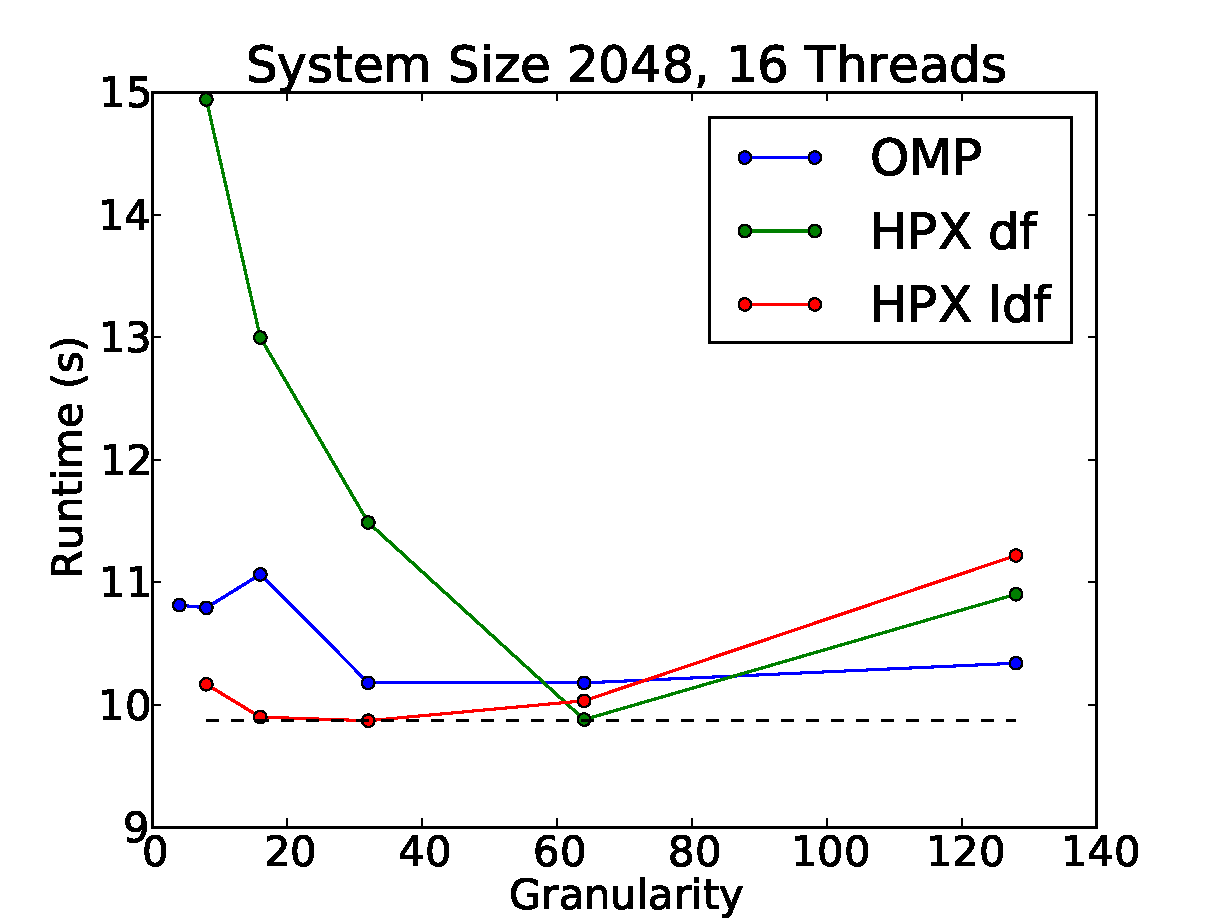
\includegraphics[width=\textwidth]{../plot/trillian_granularity_16.pdf}\hfill
  \caption{Granularity with 16 Threads.} 
  \label{fig:granularity_16}
 \end{subfigure}
 \begin{subfigure}[b]{0.49\textwidth}
  \centering
  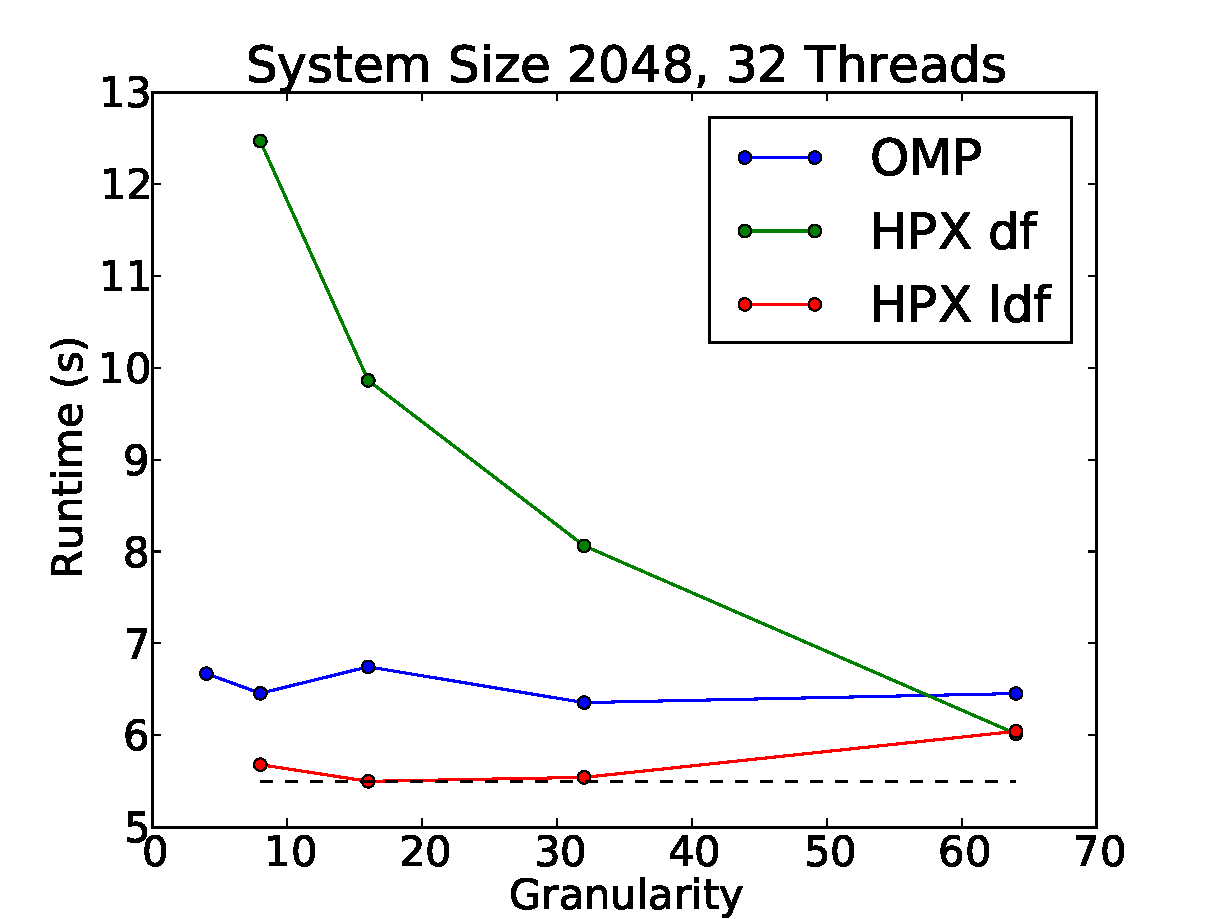
\includegraphics[width=\textwidth]{../plot/trillian_granularity_32.pdf}\hfill
  \caption{Granularity with 32 Threads.} 
  \label{fig:granularity_32}
 \end{subfigure}
 \caption{Granularity dependence of the run-time of the simulation on 16 (a) and 32 (b) Threads on a 4xOpteron6272 Machine (64 Cores). The granularity is the number of rows per task in the 2D simulation.}
\end{figure}

\begin{figure}
 \begin{subfigure}[b]{0.49\textwidth}
  \centering
  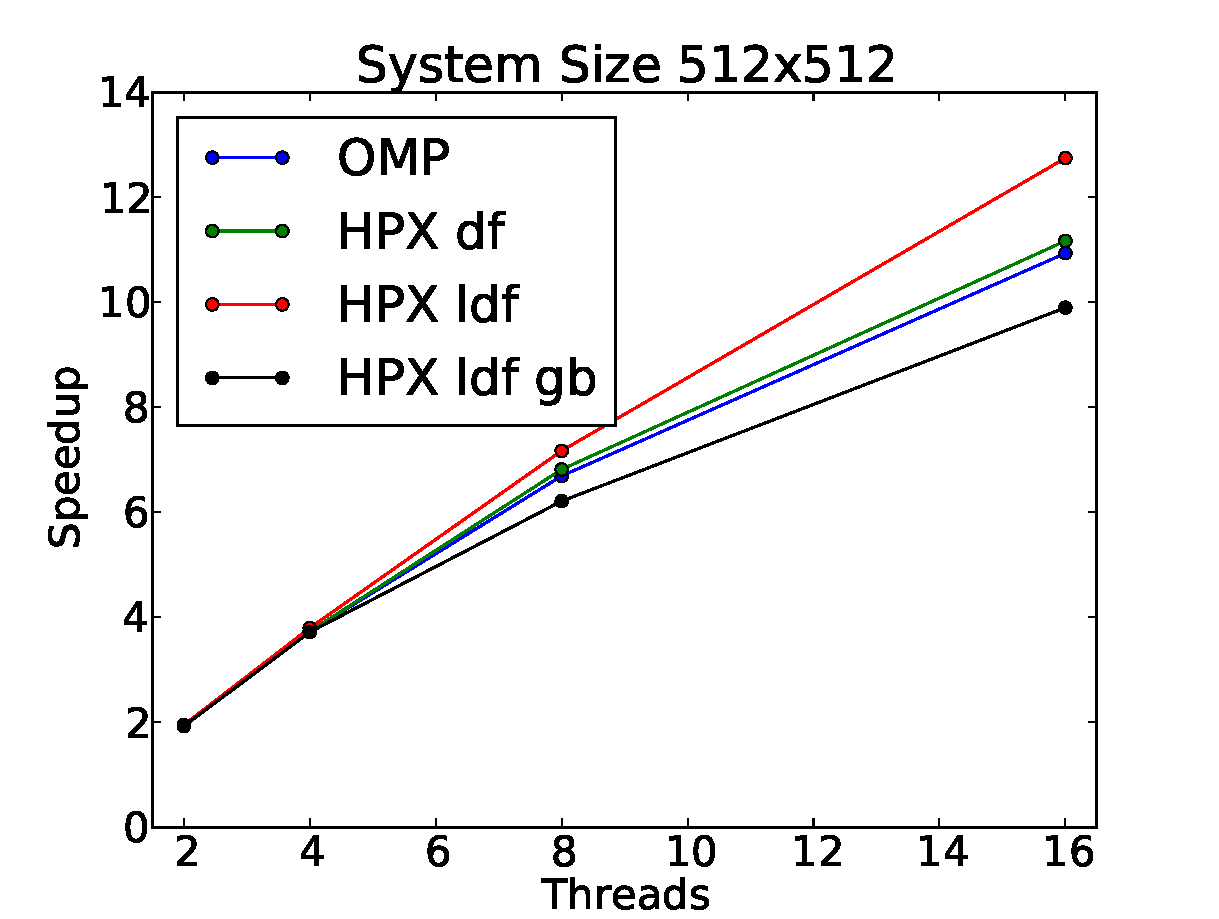
\includegraphics[width=\textwidth]{../plot/marvin_scaling_512.pdf}\hfill
  \caption{Performance with 512x512 lattice sites.} 
  \label{fig:scaling_marvin_512}
 \end{subfigure}
 \begin{subfigure}[b]{0.49\textwidth}
  \centering
  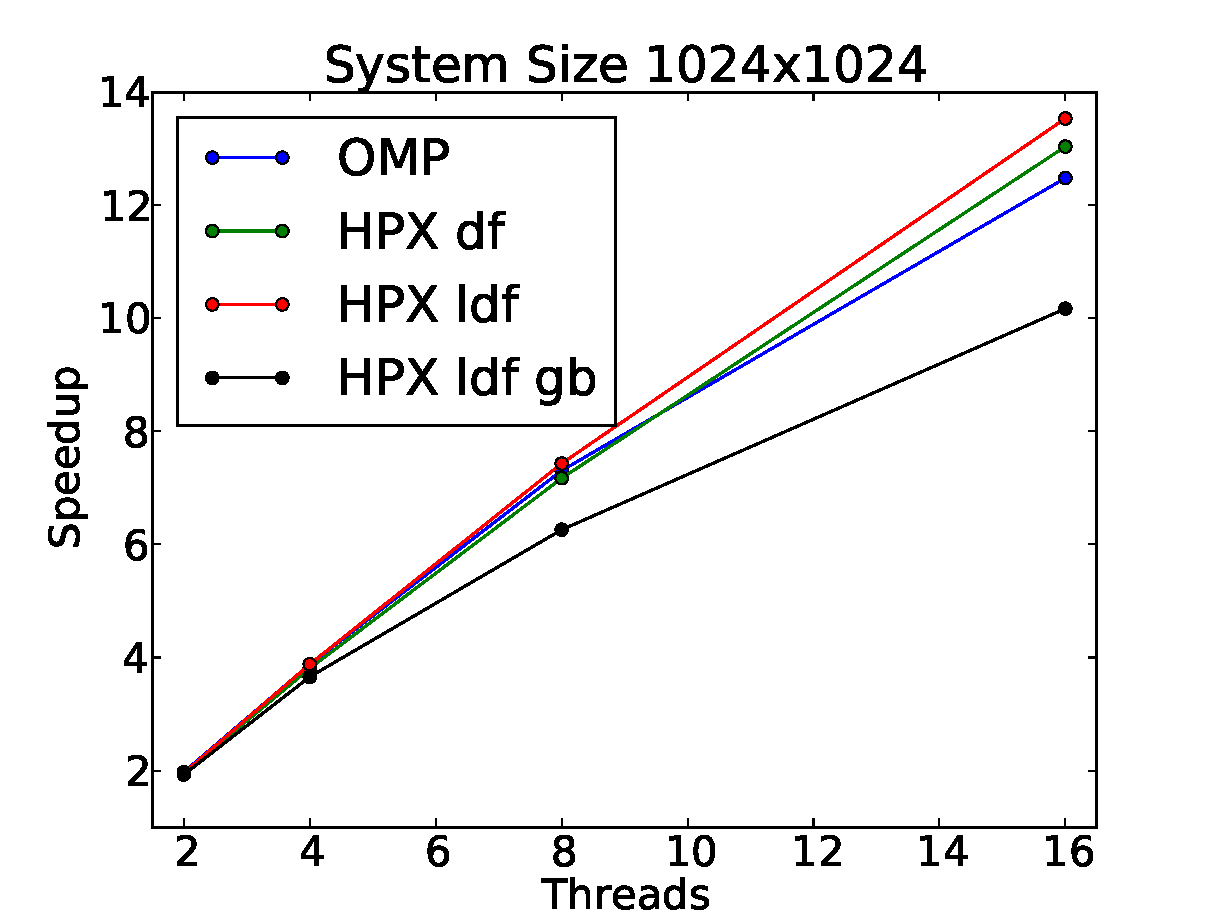
\includegraphics[width=\textwidth]{../plot/marvin_scaling_1024.pdf}\hfill
  \caption{Performance with 1024x1024 lattice sites.} 
  \label{fig:scaling_marvin_1024}
 \end{subfigure}
 \caption{Strong scaling for a system of size 512x512 (a) and 1024x1024(b) on a 2xXeonE5-2450 with 16 Cores (no Hyperthreading). The black curve (``HPX ldf gb'') represents the performance of a simulation using HPX local dataflows with additional global barriers.}
\end{figure}

\begin{figure}
 \begin{subfigure}[b]{0.49\textwidth}
  \centering
  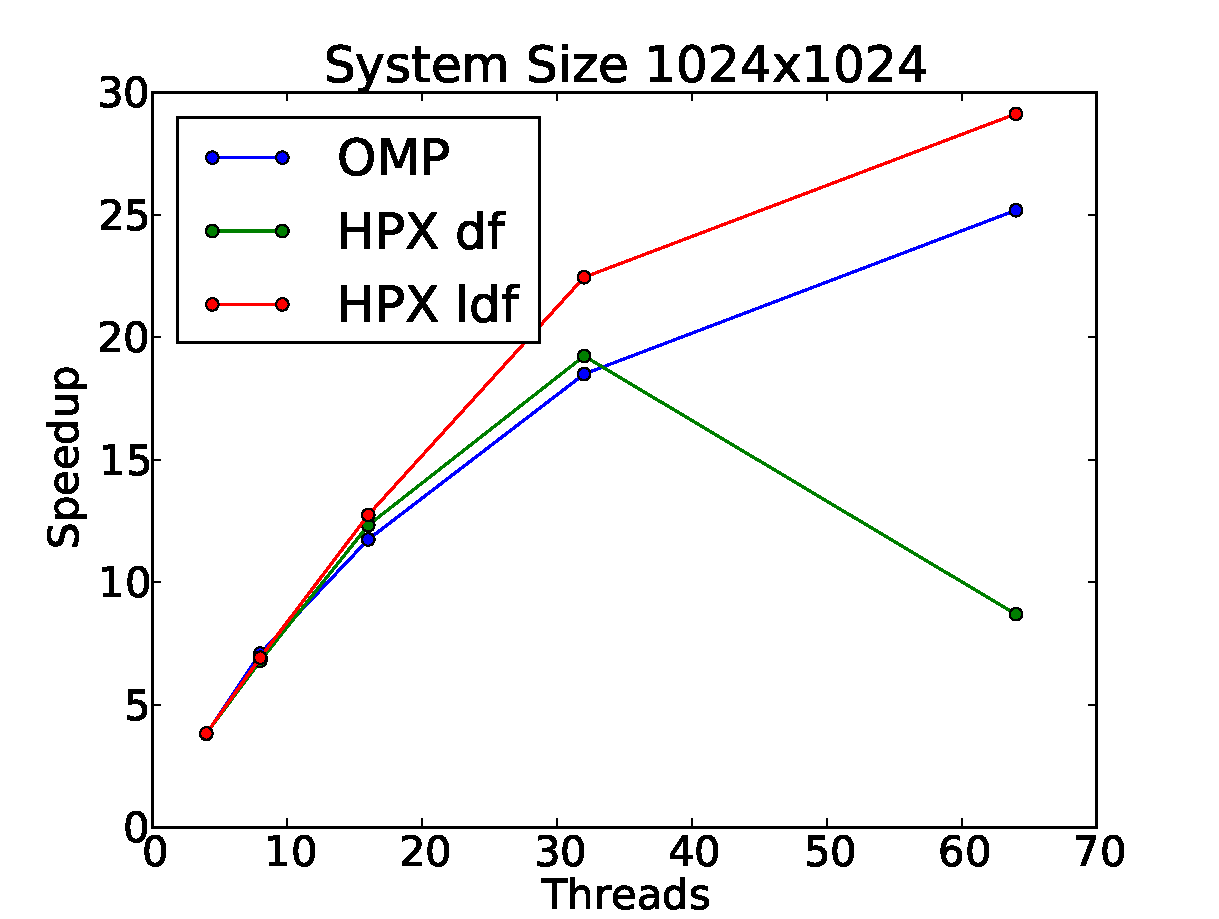
\includegraphics[width=\textwidth]{../plot/trillian_scaling_1024.pdf}\hfill
  \caption{Performance with 1024x1024 lattice sites.} 
  \label{fig:scaling_trillian_1024}
 \end{subfigure}
 \begin{subfigure}[b]{0.49\textwidth}
  \centering
  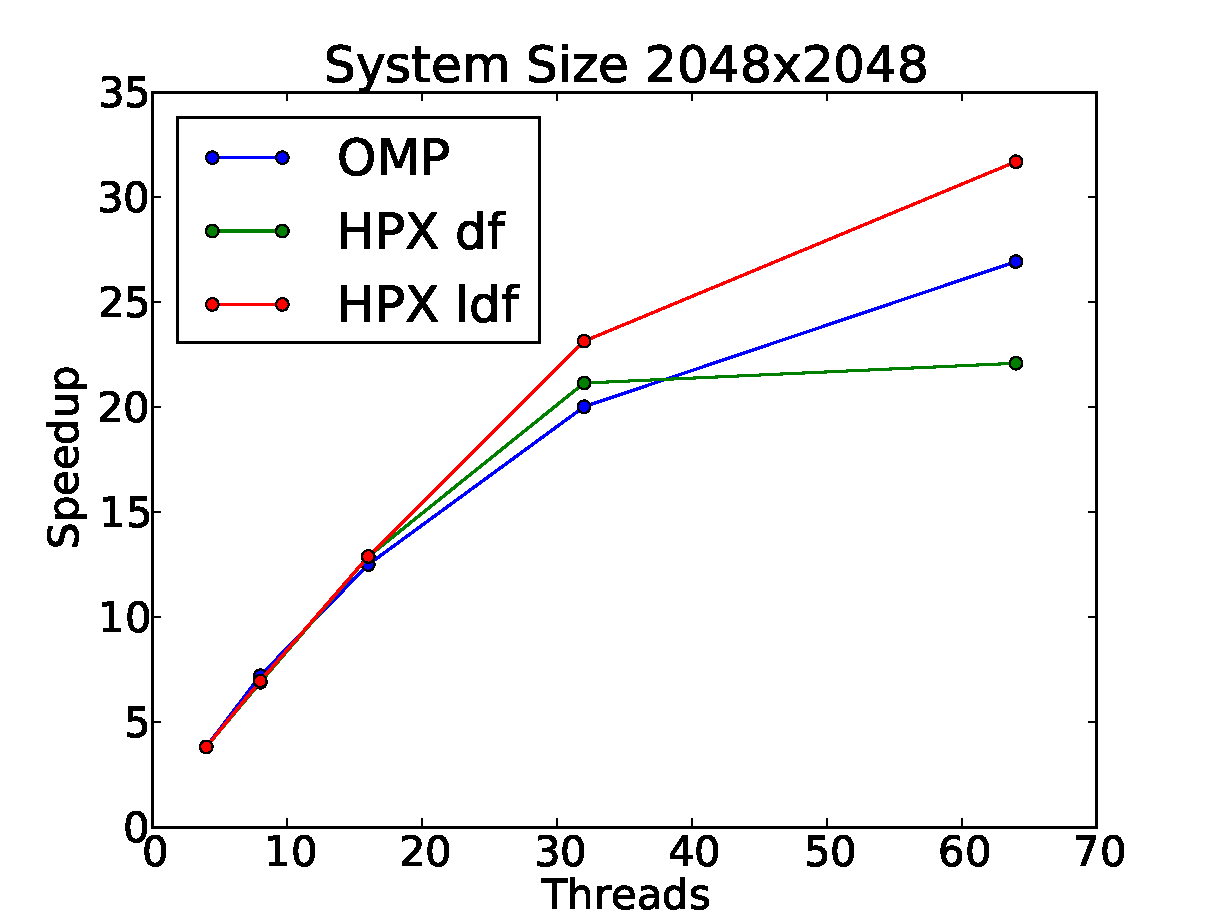
\includegraphics[width=\textwidth]{../plot/trillian_scaling_2048.pdf}\hfill
  \caption{Performance with 2048x2048 lattice sites.} 
  \label{fig:scaling_trillian_2048}
 \end{subfigure}
 \caption{Strong scaling for a system of size 1024x1024 (a) and 2048x2048(b) on a 4xOpteron6272 (64 Cores).}
\end{figure}

\end{document}          
